\documentclass[12pt]{article}
\usepackage{amssymb,mathrsfs, amsmath,amsfonts}
\usepackage{mathtools}
\usepackage{graphicx}
\usepackage{enumitem}
\usepackage{braket}
\graphicspath{ {./ps5-assets/}{./exercises/handwritten/ps5/ps5-assets/} }
\title{Problem Set 5}
\author{CSE 468}
\date{May 2021}
%%
%%
\newcommand{\Blank}{\mbox{\hskip 4pt\vrule width 1in depth 2pt}\vrule width 0pt height 2.0em}
\newcommand{\NameBlank}{\mbox{\hskip 4pt\vrule width 2.5in depth 2pt}\vrule width 0pt height 2.0em}
%%
%% Leave at least #1 space, default to what is below
%%
\def\DefaultSpace{1in}
\newcommand{\LeaveSpace}[1][\DefaultSpace]{%
\vskip #1 plus 1fil\relax\hbox to 0pt{\hss} %
}

\begin{document}
\maketitle

\noindent Name:\NameBlank{} \newline
\noindent Student ID:\NameBlank{} \newline
\textbf{Note:} You may discuss these problems with other students, but you must write your own solutions.

\begin{enumerate}[font=\bfseries]
    \item \[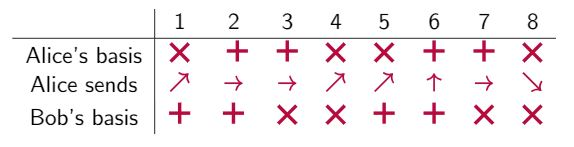
\includegraphics[scale=0.8]{bb84_q1}\]
    (3 points) Calculate Alice and Bob's shared key based on the table above and the BB84 protocol described in class.
    \item \[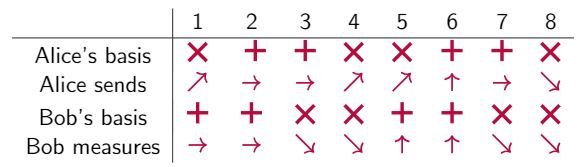
\includegraphics[scale=0.8]{bb84_q2}\]
    (5 points) Now consider the same table with one additional row, Bob's measurements. Is Eve present? If so, how can you tell? If not, why not?
    \item (3 points) Consider the BB84 protocol. Why must Alice wait until after Bob has measured all states before publishing the bases she measured in?
    \item (3 points) What is the minimum number of measurements Alice and Bob must publish in order to be at least 90\% confident Eve is not present?
    \item (6 points) Suppose you and your friend Bob are trying to decide between using the E91 and BB84 protocols. What factors should you take into account? When would you prefer one protocol over the other?
    \item (2 points) What is the primary property of quantum mechanics that enables the BB84 protocol?
    \item (2 points) What is the primary property of quantum mechanics that enables the E91 protocol?
    \item (20 points) Consider a variation on the BB84 protocol. In this protocol, Alice only has two possible states to send to Bob (as opposed to 4 in BB84). Alice will either send $\uparrow$ or $\nearrow$ to Bob. Bob will measure in either the $+$ or $\times$ basis. Let's explore how Alice and Bob can generate a shared key using these constraints.
        \begin{enumerate}
            \item Suppose Alice sends $\uparrow$ and Bob measures in the $+$ basis. What are the possible measurement outcomes for Bob?
            \item Suppose Alice sends $\nearrow$ and Bob measures in the $\times$ basis. What are the possible measurement outcomes for Bob?
            \item Suppose Alice sends $\uparrow$ and Bob measures in the $\times$ basis. What are the possible measurement outcomes for Bob?
            \item Suppose Alice sends $\nearrow$ and Bob measures in the $+$ basis. What are the possible measurement outcomes for Bob?
            \item Regardless of basis, what does Bob know about the initial state Alice sent if he measures $\uparrow$ ? What if he measures $\nearrow$ ? What if he measures  $\rightarrow$ ? What if he measures $\nwarrow$ ?
            \item Describe how Alice and Bob could construct a shared key based on the above observations. You can decide which symbol corresponds to each 0 and 1. 
            \item How could Alice and Bob detect Eve?
        \end{enumerate}
    \item \[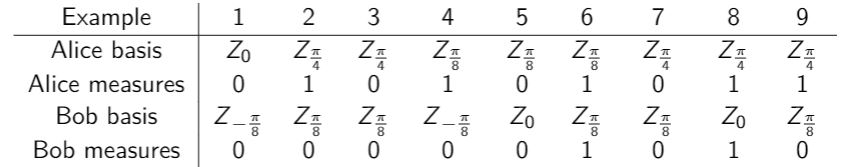
\includegraphics[scale=0.8]{e91_table}\]
    (5 points) Consider the above example of the E91 protocol. Is Eve present? Why or why not?
    \item (3 points) Give a valid strategy for Alice and Bob to ``destroy'' their qubits before publishing their bases so that Eve cannot discover their shared key. 
    \item One or two CHSH questions
    \item (Bonus, up to 3 points) Write one interesting question related to the content of this homework, and indicate the correct answer. The question can be multiple-choice or free-response.  Interesting questions get credit here;  sufficiently good questions might appear on an exam.
\end{enumerate}



\end{document}